\chapter{Datasets and Trigger Paths}\label{ch:appendix_datasets_triggerpaths}
\RaggedRight \parindent=25pt
Events containing two prompt photon events are selected online with \texttt{HLT\_DoublePhoton60} or \texttt{HLT\_DoublePhoton70} trigger paths for 2016 and 2017/2018 data respectively. These two triggers require at least two reconstructed photon candidates with a transverse momentum $p_{T} > 60 (70)$~GeV across the range $|\eta| < 3.0$. At this level, the primary selection requires that each photon candidate must have a ratio of the hadronic to the electromagnetic energy (H/E) $<$ 0.15. The electromagnetic energy here is defined as the corrected supercluster energy while the hadronic energy is the total HCAL energy within a cone of $\Delta R <$  0.15 from the supercluster position. This ratio is also the amount of the HCAL energy in the tower directly behind the photon seed crystal. This trigger is seeded by the logical \texttt{OR} of a suite \texttt{SingleEG}, \texttt{DoubleEG}, \texttt{SingleJet}, and \texttt{SingleTau} L1 seeds with varying trigger thresholds. 

% To quantify the efficiency of the \texttt{HLT_DoublePhoton60/70} triggers, we normalized using the reference trigger \texttt{HLT_DoublePhoton33_CaloIdL}. This trigger selects events with two photons, each having transverse momentum greater than 33 GeV and satisfying the Calorimeter Identification (CaloId) criteria. The efficiency primarily depends on the transverse momentum ($p_{T}$) of the second-leading photon, which is the photon with the second highest $p_{T}$ among the collection. The results of this analysis are presented in Figure~\ref{fig:trigger_efficiency}. Previous studies \cite{ref:AN2016_167} have demonstrated that there are no additional sources of efficiency, and this study serves as a cross-check.

To quantify the efficiency of the \texttt{HLT\_DoublePhoton60/70} triggers, we used the reference trigger \texttt{HLT\_DoublePhoton33\_CaloIdL} for normalization. The latter trigger selects events that contain two photons, each with transverse momentum greater than 33 GeV and satisfying the Calorimeter Identification (CaloId) criteria. The efficiency is primarily a function of the $p_{T}$ of the second-leading photon, the photon which has the second highest $p_{T}$ among the collection of photons. The results are shown in Figure~\ref{fig:trigger_efficiency}. This procedure only probes the turn-on of the $p_{T}$ leg \cite{ref:AN2016_167} have shown that there is no additional source of efficiency and this study serves as a cross-check. 

Additionally, we use \texttt{HLT\_ECALHT800} as a backup trigger which adds approximately 0.2$\%$ in yield across the entire 2016-2018 data set. Although this comprises only a small fraction of the total event yield, we choose to use it anyway in cases where the diphoton triggers lose efficiency specifically at high diphoton invariant masses. We calculate only the yield over the full analysis region with several thousand events, without viewing any distributions to avoid bias during the blinded phase of the analysis. The trigger efficiency is fully efficient at $p_T > 125$ GeV, which is the photon $p_{T}$ selection used in this analysis. 

% % generated by Tools/bin/efficiency.cc
% \begin{figure}[tbp!]
% \begin{center}
% %\includegraphics[angle=0,width=0.4\textwidth]{figures/eff2015.pdf}
% 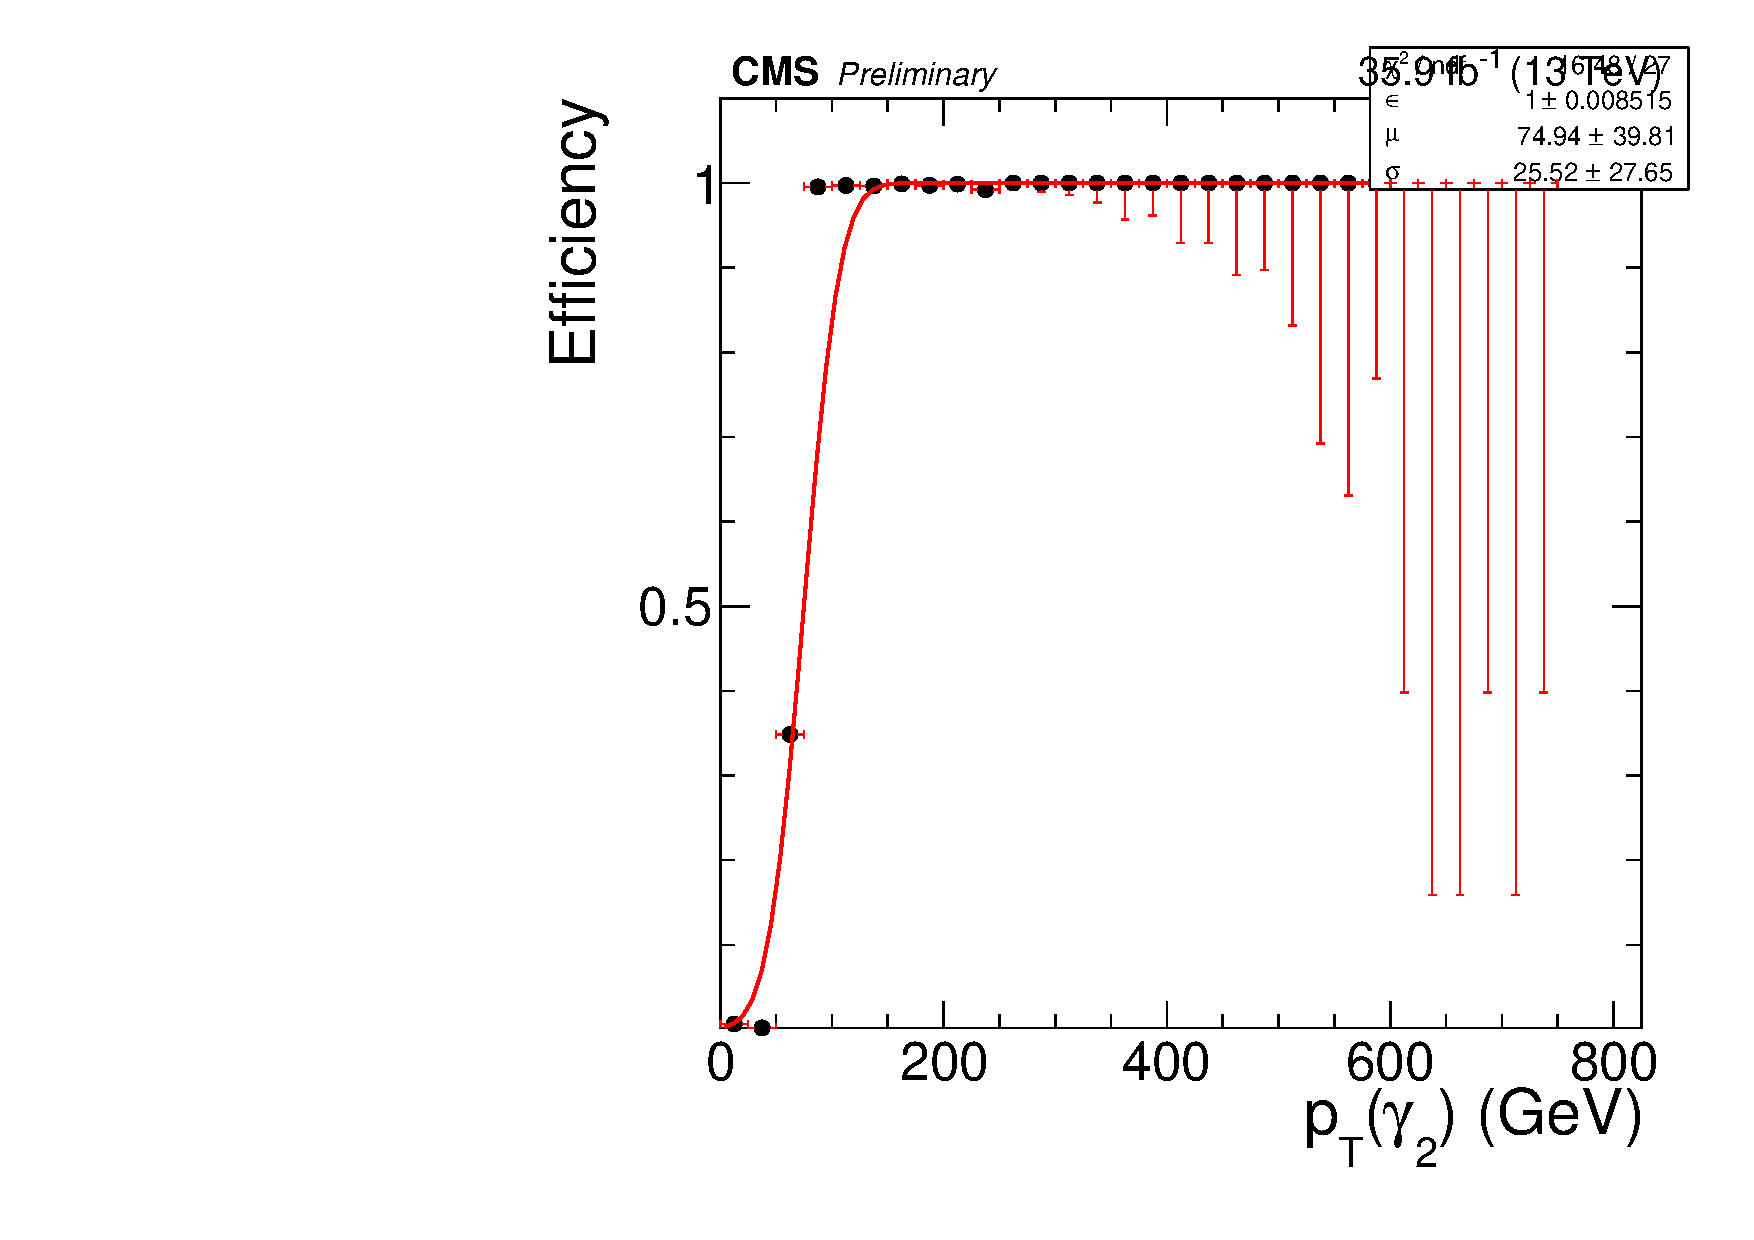
\includegraphics[angle=0,width=0.3\textwidth]{fig/eff_2016_Photon2_pt.pdf}
% 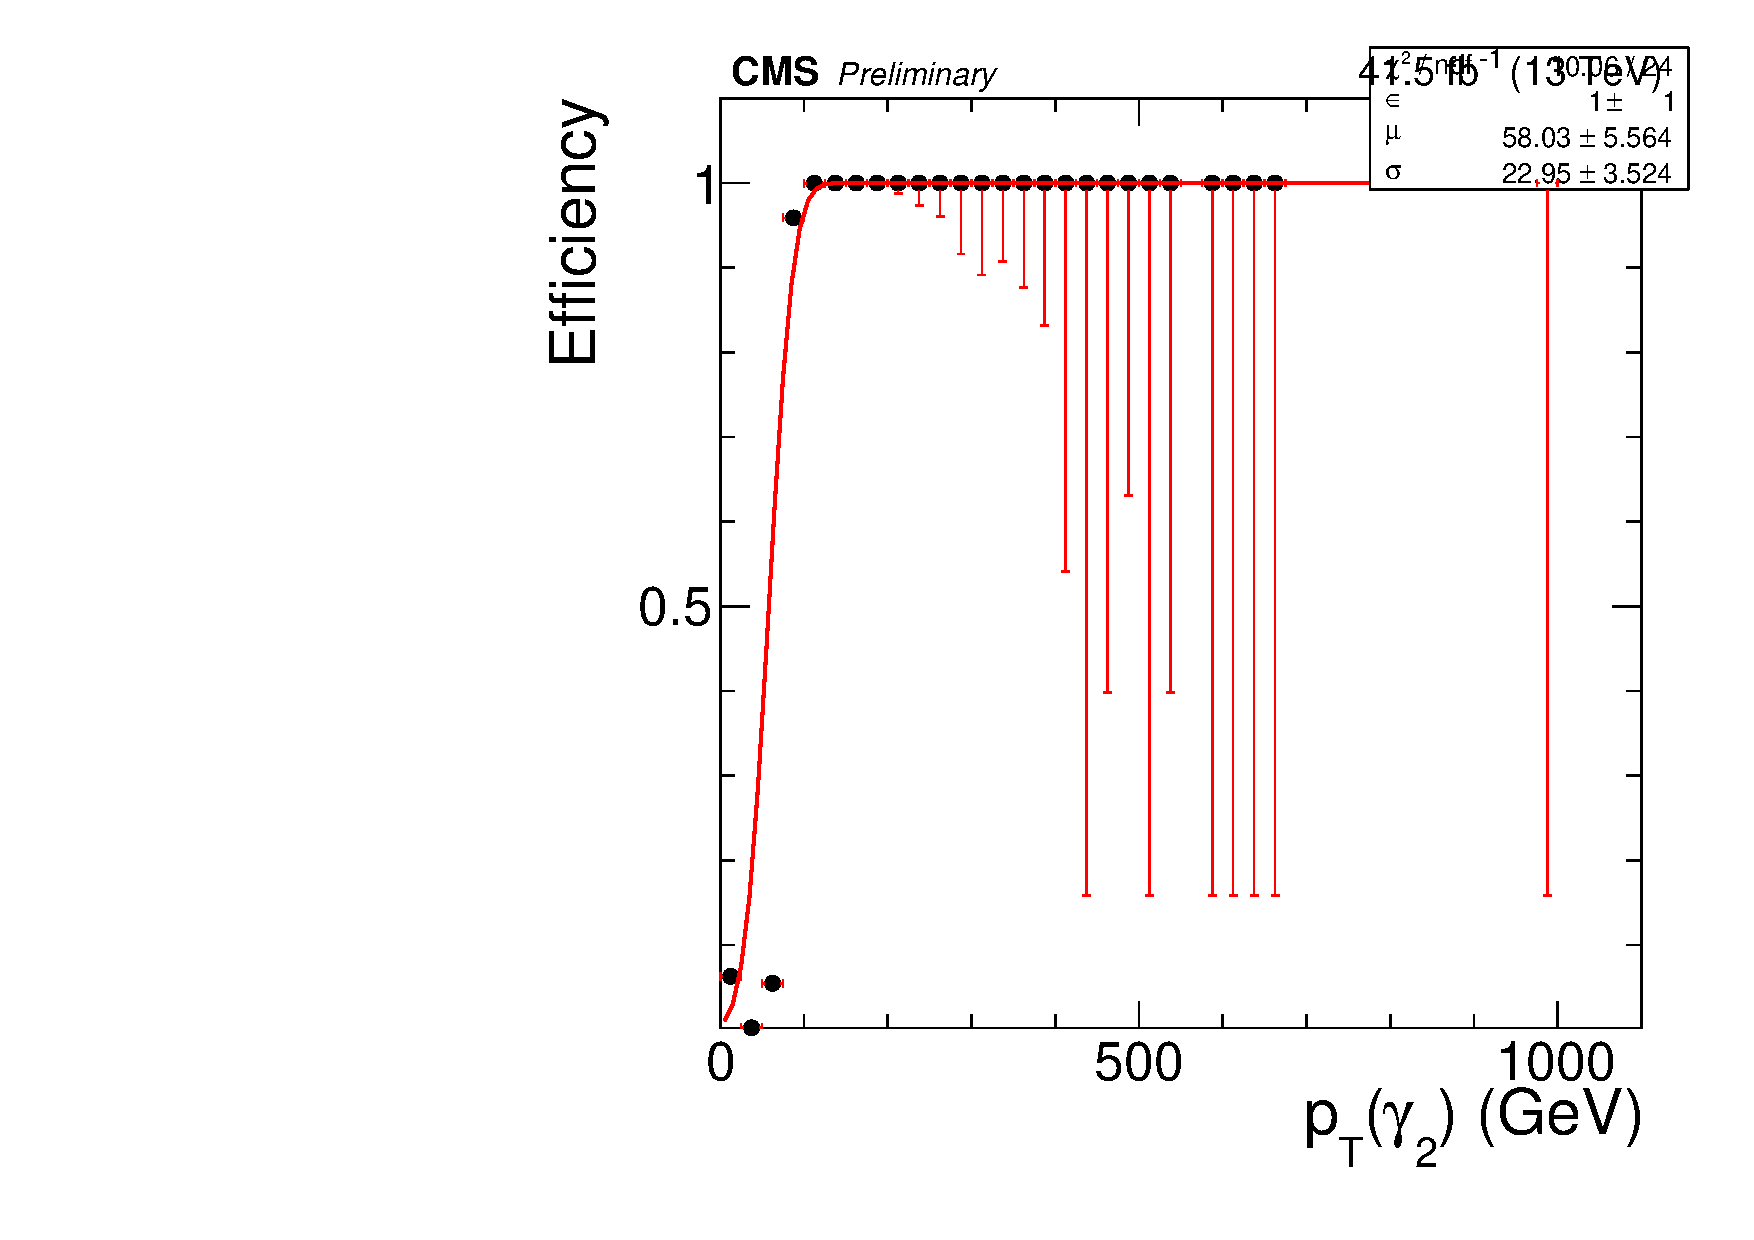
\includegraphics[angle=0,width=0.3\textwidth]{fig/eff_2017_Photon2_pt.pdf}
% 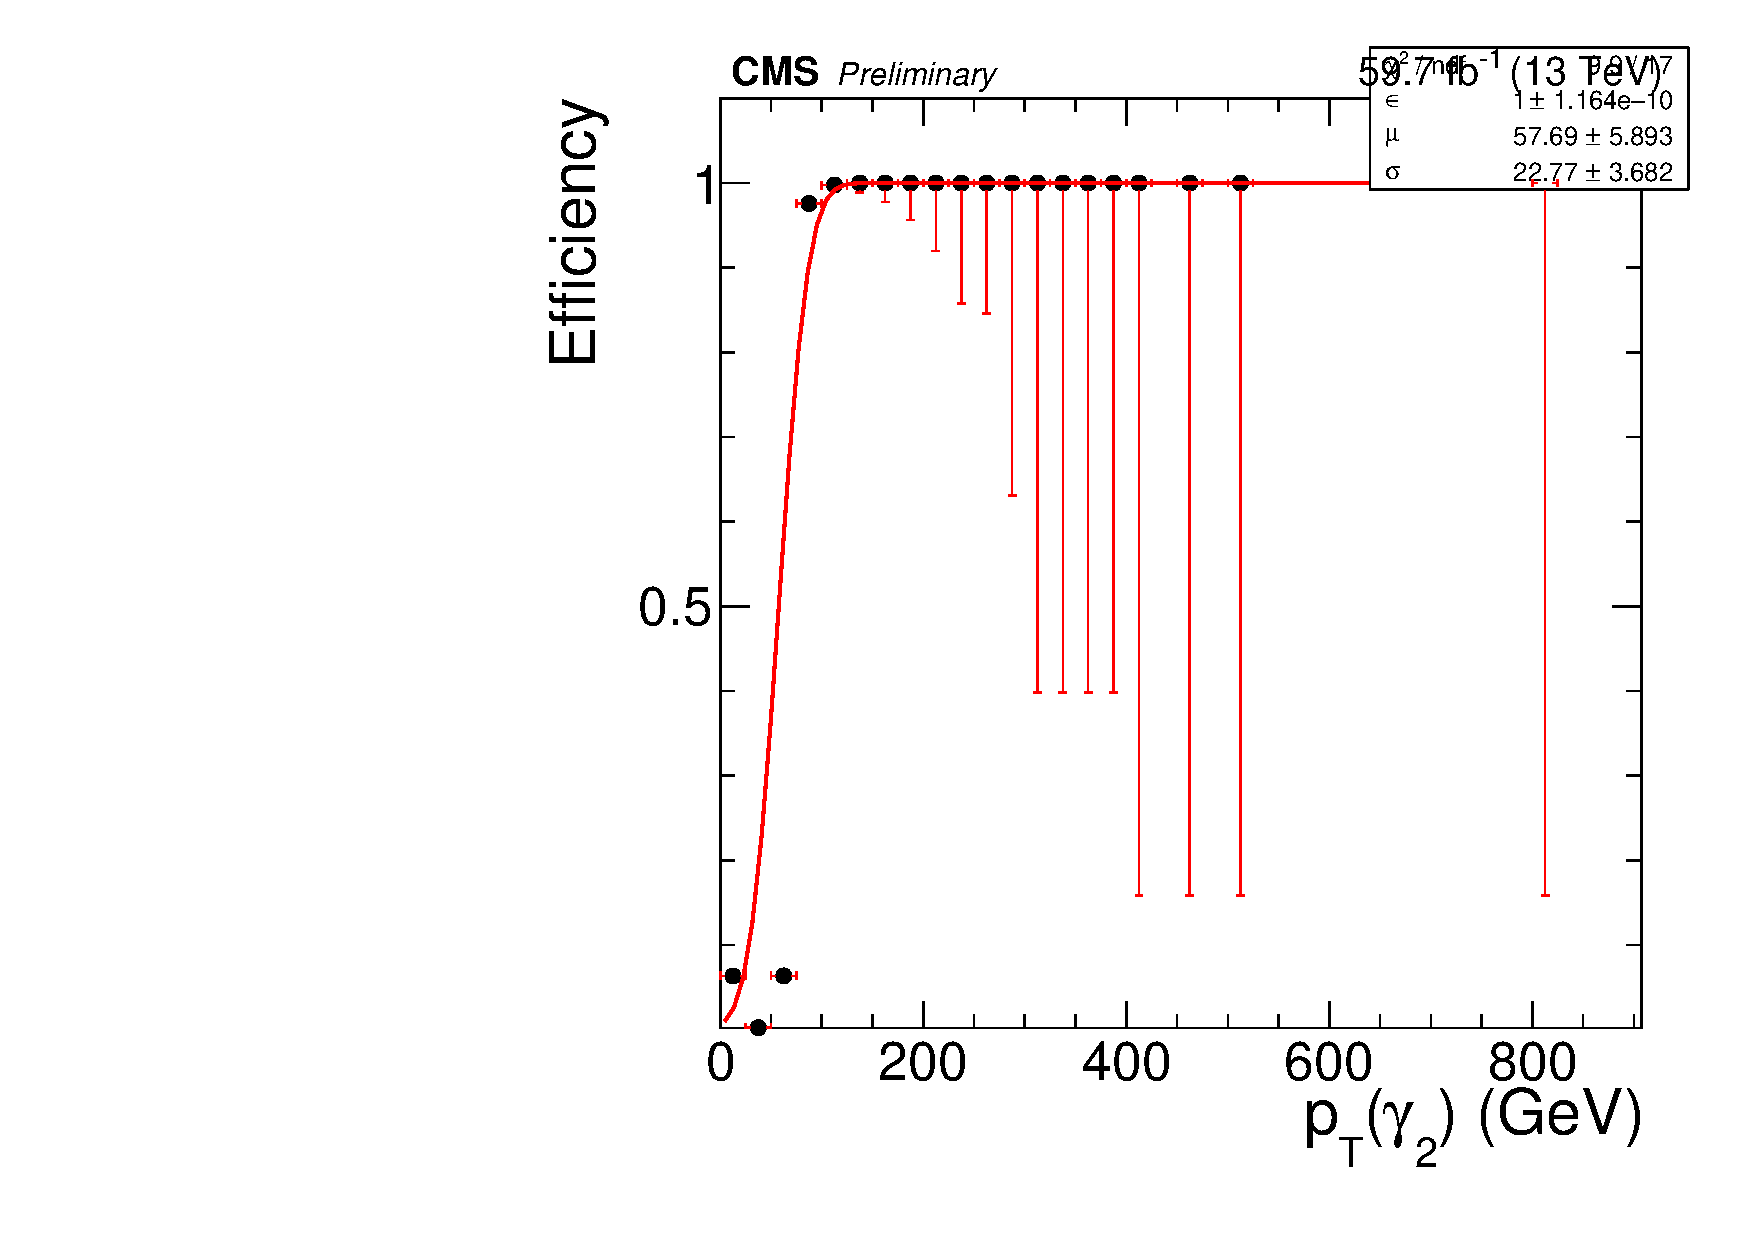
\includegraphics[angle=0,width=0.3\textwidth]{fig/eff_2018_Photon2_pt.pdf}
% \end{center}
% \caption{Efficiency of \texttt{HLT\_DoublePhoton60} (2016) or \texttt{HLT\_DoublePhoton70} (2017--2018) trigger (measured with reference trigger the \texttt{HLT\_DoublePhoton33\_CaloIdL}) as a function of the \pt of the second-leading photon in 2016 (left), 2017 (center) and 2018 (right) data. The precise form of the fit is irrelevant as the efficiency plateaus well before the offline cut value.}
% \label{fig:trigger_efficiency}
% \end{figure}
\section{Data Samples}~\label{Data samples}
The data samples considered for this analysis are listed in Table~\ref{table:datasets2016-18} and correspond to an integrated luminosity of 138~\fbinv collected by the CMS experiment from 2016 to the end of 2018. The 2016 and 2017 data sets were processed in {\tt CMSSW\_9\_4\_13}, while the 2018 data sets are processed using {\tt CMSSW\_10\_2\_16}. The global tags used to analyze the data are listed in Table~\ref{table:datasets2016-18}. These samples also fulfill standard data quality criteria for all the subdetectors of CMS as specified by the good run JSONs listed in Table~\ref{table:json}. Calculation of the luminosity using the \texttt{HLT\_ECALHT800} trigger gives the same luminosity. The integrated luminosity of the MINIAOD Data samples where calculated with the \texttt{--hltpath HLT\_DoublePhoton60/70} option of \texttt{brilcalc} and the processed luminosity sections given by \texttt{crab --report}.

%brilcalc lumi --normtag ~lumipro/public/Normtags/normtag DATACERT.json -i JSON 2017/8 data.
% \begin{table}[!htbp]
% 	\caption{MINIAOD Data samples analyzed and the corresponding integrated luminosity, calculated with the \texttt{--hltpath HLT\_DoublePhoton60/70} option of \texttt{brilcalc} and the processed luminosity sections given by \texttt{crab --report}.}

\begin{table}[!htbp]
	\caption{MINIAOD Data samples analyzed and the corresponding integrated luminosity, calculated with Double Photon Trigger and the processed luminosity sections.}
	
	\centering
	\resizebox{\textwidth}{!}{%
	\vspace{\baselineskip}
	\begin{tabular}{lcc}
	\hline \hline
	Data set & Int. lumi (\fbinv) & Global tag\\
	\hline
	/DoubleEG/Run2016B-17Jul2018\_ver2-v1 & 5.781 &  94X\_dataRun2\_v10 \\
	/DoubleEG/Run2016C-17Jul2018\_v1      & 2.573 &  94X\_dataRun2\_v10 \\
	/DoubleEG/Run2016D-17Jul2018\_v1      & 4.248 &  94X\_dataRun2\_v10 \\
	/DoubleEG/Run2016E-17Jul2018\_v1      & 4.009 &  94X\_dataRun2\_v10 \\
	/DoubleEG/Run2016F-17Jul2018\_v1      & 3.102 &  94X\_dataRun2\_v10 \\
	/DoubleEG/Run2016G-17Jul2018\_v1      & 7.540 &  94X\_dataRun2\_v10 \\
	/DoubleEG/Run2016H-17Jul2018\_v1      & 8.606 &  94X\_dataRun2\_v10 \\
        2016 total integrated luminosity      & 35.86 &  \\
        \hline
        /DoubleEG/Run2017B-31Mar2018\_v1      & 4.79 &  94X\_dataRun2\_v11 \\
        /DoubleEG/Run2017C-31Mar2018\_v1      & 9.63 &  94X\_dataRun2\_v11 \\
        /DoubleEG/Run2017D-31Mar2018\_v1      & 4.25 &  94X\_dataRun2\_v11 \\
        /DoubleEG/Run2017E-31Mar2018\_v1      & 9.31 &  94X\_dataRun2\_v11 \\
        /DoubleEG/Run2017F-31Mar2018\_v1      & 13.54 &  94X\_dataRun2\_v11 \\
        2017 total integrated luminosity      & 41.53 &  \\
        \hline
	/EGamma/Run2018A-17Sep2018-v2         & 13.70 & 102X\_dataRun2\_v11 \\
	/EGamma/Run2018B-17Sep2018-v1         & 7.06  & 102X\_dataRun2\_v11 \\
	/EGamma/Run2018C-17Sep2018-v1         & 6.89  & 102X\_dataRun2\_v11 \\
        /EGamma/Run2018D-22Jan2019-v2/MINIAOD & 31.74 & 102X\_dataRun2\_Prompt\_v11\\
        2018 total integrated luminosity      & 59.40 &  \\
	% \hline
  % \hline

	\hline \hline
	\end{tabular}}
	\label{table:datasets2016-18}
\end{table}
% \end{landscape}

% \begin{landscape}
\begin{table}[!htbp]
	\caption{Good run JSONs used for each data period.}
	\centering
	\vspace{\baselineskip}
	\resizebox{\textwidth}{!}{%
	\begin{tabular}{lc}
	\hline \hline
	Data period & Good run JSON \\
	\hline

        2016 & Collisions16/13TeV/ReReco/Final/Cert\_271036-284044\_13TeV\_23Sep2016ReReco\_Collisions16\_JSON.txt \\
	2017 & Collisions17/13TeV/ReReco/Final/Cert\_294927-306462\_13TeV\_EOY2017ReReco\_Collisions17\_JSON\_v1.txt \\
	2018 & Collisions18/13TeV/ReReco/Final/Cert\_314472-325175\_13TeV\_17SeptEarlyReReco2018ABC\_PromptEraD\_Collisions18\_JSON.txt   \\

	\hline \hline
	\end{tabular}}
	\label{table:json}
\end{table}

%%%%%%%%%
\section{SM Prompt Diphoton Background Datasets}~\label{MCPromptBackground}

The Standard Model prompt diphoton background are listed in Tab.~\ref{table:mcbackgroundsamples}. The campaigns and global tags used to generate the ntuples are listed in Tab.~\ref{table:mcdatasets2016-18}. Here XXX stands for RunIISummer16MiniAODv3-PUMoriond17\_94X\_mcRun2\_asymptotic\_v3 for 2016 samples, RunIIFall17MiniAODv2-PU2017\_12Apr2018\_94X\_mc2017\_realistic\_v14 for 2017 samples or RunIIAutumn18MiniAOD-102X\_upgrade2018\_realistic\_v15-v1 for 2018 samples.

\begin{landscape}
\begin{table}[!htbp]
       \caption{MC background samples used in the analysis. 
       %YYY for RunIIFall17MiniAOD-94X\_mc2017\_realistic\_v10All
   % ZZZ for RunIIFall17MiniAODv2-PU2017\_12Apr2018\_94X\_mc2017\_realistic\_v14/.
       }
       \centering
       \vspace{\baselineskip}
       \begin{tabular}{lc}
       \hline \hline
       Object or process & Data set path & Cross-section (pb) \\
       \hline
  /GG\_M-500To1000\_Pt70\_TuneCP2\_13TeV-pythia8/XXX\ & 1.344e-01  \\
  /GG\_M-1000To2000\_Pt70\_TuneCP2\_13TeV-pythia8/XXX\ & 1.359e-02  \\
  /GG\_M-2000To4000\_Pt70\_TuneCP2\_13TeV-pythia8/XXX\ & 6.696e-04  \\
  /GG\_M-4000To6000\_Pt70\_TuneCP2\_13TeV-pythia8/XXX\ & 8.757e-06 \\
  \hline
  % GJets
  % $\PGg+jets$ $<H_T<$ GJets_HT-40To100_TuneCP5_13TeV-madgraphMLM-pythia8/crab_GJets_HT-40To100_TuneCP5_13TeV-madgraphMLM-pythia8__RunIIFall17MiniAOD-1core_94X_mc2017_realistic_v \\
  /GJets\_HT-40To100\_TuneCP5\_13TeV-madgraphMLM-pythia8/XXX & 1.862e+04 \\
  /GJets\_HT-100To200\_TuneCP5\_13TeV-madgraphMLM-pythia8/XXX & 8.625e+03 \\
  /GJets\_HT-200To400\_TuneCP5\_13TeV-madgraphMLM-pythia8/XXX & 2.194e+03 \\
  /GJets\_HT-400To600\_TuneCP5\_13TeV-madgraphMLM-pythia8/XXX & 2.583e+02 \\
  /GJets\_HT-600ToInf\_TuneCP5\_13TeV-madgraphMLM-pythia8/XXX & 8.520e+01 \\
  \hline
  % GGJets
 /GGJets\_M-60To200\_Pt-50\_13TeV-sherpa/XXX & 5.785e+00 \\
 /GGJets\_M-200To500\_Pt-50\_13TeV-sherpa/XXX &  2.244e+00 \\
 /GGJets\_M-500To1000\_Pt-50\_13TeV-sherpa/XXX & 1.510e-01  \\
 /GGJets\_M-1000To2000\_Pt-50\_13TeV-sherpa/XXX & 1.084e-02 \\
 /GGJets\_M-2000To4000\_Pt-50\_13TeV-sherpa/XXX &  3.690e-04 \\
 /GGJets\_M-4000To6000\_Pt-50\_13TeV-sherpa/XXX &  2.451e-06 \\
 /GGJets\_M-6000To8000\_Pt-50\_13TeV-sherpa/XXX &  1.753e-08 \\
 /GGJets\_M-8000To13000\_Pt-50\_13TeV-sherpa/XXX &  7.053e-11\\
       \hline \hline
       \end{tabular}
    %   \label{table:sherpaDiphoton}
       \label{table:mcbackgroundsamples}
\end{table}
\end{landscape}

\begin{table}[!htbp]
  \caption{For each year, the campaign in which MC samples were generated and the global tag used to generate the analysis ntuples.
}
  \centering
  \vspace{\baselineskip}
  \begin{tabular}{lcc}
  \hline \hline
  Year & Campaign & Global tag\\
  \hline
        2016 & RunIISummer16MiniAODv3 & \texttt{94X\_dataRun2\_v10}\\
        2017 & RunIIFall17MiniAODv2   & \texttt{94X\_dataRun2\_v11}\\
        2018 & RunIIAutumn18MiniAOD   & \texttt{102X\_dataRun2\_v11}\\
  \hline \hline
  \end{tabular}
  \label{table:mcdatasets2016-18}
\end{table}

%%%%%%%%
\section{Fake Rate Datasets}~\label{FakeRateDatasets}
Table~\ref{table:dset-JetHTFakeRate} and Table~\ref{table:dset-DoubleMuonFakeRate} lists the jet-triggered and muon-triggered datasets, respectively, that were used for the derivation of the fake rate.

\begin{table}[!htbp]
	\caption{The \JetHT Datasets used for constructing the fake templates and for deriving the fake rates. The fake rate is derived from the average of the rates obtained independently from the \JetHT and \DoubleMuon dataset}
	\centering
	\resizebox{0.8\textwidth}{!}{%
	\vspace{\baselineskip}
	\begin{tabular}{l}
	\hline \hline
	Data set \\
	\hline
{\small
  /JetHT/Run2016B-17Jul2018\_ver1-v1/MINIAOD \\
  /JetHT/Run2016B-17Jul2018\_ver2-v2/MINIAOD \\
  /JetHT/Run2016C-17Jul2018-v1/MINIAOD  \\
  /JetHT/Run2016D-17Jul2018-v1/MINIAOD  \\
  /JetHT/Run2016E-17Jul2018-v1/MINIAOD  \\
  /JetHT/Run2016F-17Jul2018-v1/MINIAOD  \\
  /JetHT/Run2016G-17Jul2018-v1/MINIAOD  \\
  /JetHT/Run2016H-17Jul2018-v1/MINIAOD  \\
  \hline
  /JetHT/Run2017B-31Mar2018-v1/MINIAOD \\
  /JetHT/Run2017C-31Mar2018-v1/MINIAOD \\
  /JetHT/Run2017D-31Mar2018-v1/MINIAOD \\
  /JetHT/Run2017E-31Mar2018-v1/MINIAOD \\
  /JetHT/Run2017F-31Mar2018-v1/MINIAOD \\
  \hline
  /JetHT/Run2018A-17Sep2018-v1/MINIAOD \\
  /JetHT/Run2018B-17Sep2018-v1/MINIAOD \\
  /JetHT/Run2018C-17Sep2018-v1/MINIAOD \\
  /JetHT/Run2018D-PromptReco-v2/MINIAOD \\
}
	\hline \hline
	\end{tabular}}
	\label{table:dset-JetHTFakeRate}
\end{table}

\begin{table}[!htbp]
	\caption{The \texttt{DoubleMuon} datasets for fake rate estimation. The fake rate is derived from the average of the rates obtained independently from the \JetHT and \DoubleMuon datasets.}
	\centering
	\resizebox{0.8\textwidth}{!}{%
	\vspace{\baselineskip}
	\begin{tabular}{l}
	\hline \hline
	Data set \\
	\hline
  {\small
  /DoubleMuon/Run2016B-17Jul2018\_ver1-v1/MINIAOD \\
  /DoubleMuon/Run2016B-17Jul2018\_ver2-v1/MINIAOD \\
  /DoubleMuon/Run2016C-17Jul2018-v1/MINIAOD \\
  /DoubleMuon/Run2016D-17Jul2018-v1/MINIAOD \\
  /DoubleMuon/Run2016E-17Jul2018-v1/MINIAOD \\
  /DoubleMuon/Run2016F-17Jul2018-v1/MINIAOD \\
  /DoubleMuon/Run2016G-17Jul2018-v1/MINIAOD \\
  /DoubleMuon/Run2016H-17Jul2018-v1/MINIAOD \\
  \hline
  /DoubleMuon/Run2017B-31Mar2018-v1/MINIAOD \\
  /DoubleMuon/Run2017C-31Mar2018-v1/MINIAOD \\
  /DoubleMuon/Run2017D-31Mar2018-v1/MINIAOD \\
  /DoubleMuon/Run2017E-31Mar2018-v1/MINIAOD \\
  /DoubleMuon/Run2017F-31Mar2018-v1/MINIAOD \\
  \hline
  /DoubleMuon/Run2018A-17Sep2018-v2/MINIAOD \\
  /DoubleMuon/Run2018B-17Sep2018-v1/MINIAOD \\
  /DoubleMuon/Run2018C-17Sep2018-v1/MINIAOD \\
  /DoubleMuon/Run2018D-PromptReco-v2/MINIAOD \\
 }
	\hline \hline
	\end{tabular}}
	\label{table:dset-DoubleMuonFakeRate}
\end{table}

\section{Closure Test MC Datasets}~\label{ClosureTestMCDatasets}
The Closure test makes use of MC simulations rather than data in validating the Fake Rate method. The MC datasets used are listed in Table~\ref{table:dset-2016-closuretest} and Table~\ref{table:dset-2017-18-closuretest} for the 2016 and 2017-18, respectively. 

\begin{table}[!htbp]
  \caption{2016 MC Fakes}
  \centering
  \resizebox{\textwidth}{!}{%
  \vspace{\baselineskip}
  \begin{tabular}{lc}
  \hline \hline
  Data set & Cross section (pb)\\
  \hline
  /QCD\_Pt\_5to10\_TuneCUETP8M1 & 61018300000. \\
  /QCD\_Pt\_10to15\_TuneCUETP8M1 & 5887580000. \\
  /QCD\_Pt\_15to30\_TuneCUETP8M1 & 1837410000. \\
  /QCD\_Pt\_30to50\_TuneCUETP8M1 & 140932000. \\
  /QCD\_Pt\_50to80\_TuneCUETP8M1 & 19204300. \\
  /QCD\_Pt\_80to120\_TuneCUETP8M1 & 2762530. \\
  /QCD\_Pt\_120to170\_TuneCUETP8M1 & 471100. \\
  /QCD\_Pt\_170to300\_TuneCUETP8M1 & 117276. \\
  /QCD\_Pt\_300to470\_TuneCUETP8M1 & 7823. \\
  /QC\_Pt\_470to600\_TuneCUETP8M1 & 648.2 \\
  /QCD\_Pt\_600to800\_TuneCUETP8M1 & 186.9 \\
  /QCD\_Pt\_800to1000\_TuneCUETP8M1 & 32.293 \\
  /QCD\_Pt\_1000to1400\_TuneCUETP8M1 & 9.4183 \\
  /QCD\_Pt\_1400to1800\_TuneCUETP8M1 & 0.84265 \\
  /QCD\_Pt\_1800to2400\_TuneCUETP8M1 & 0.114943 \\
  /QCD\_Pt\_2400to3200\_TuneCUETP8M1 & 0.00682981 \\
  /QCD\_Pt\_3200toInf\_TuneCUETP8M1 & 0.000165445 \\
  /GJets\_HT-40To100\_TuneCUETP8M1\_13TeV-madgraphMLM-pythia8 & 2.121e+04 \\
  /GJets\_HT-100To200\_TuneCUETP8M1\_13TeV-madgraphMLM-pythia8 & 9.863e+03 \\
  /GJets\_HT-200To400\_TuneCUETP8M1\_13TeV-madgraphMLM-pythia8 & 2.298e+03 \\
  /GJets\_HT-400To600\_TuneCUETP8M1\_13TeV-madgraphMLM-pythia8 & 2.816e+02 \\
  /GJets\_HT-600ToInf\_TuneCUETP8M1\_13TeV-madgraphMLM-pythia8 & 9.465e+01 \\

  \hline \hline
  \end{tabular}}
  \label{table:dset-2016-closuretest}
\end{table}
% \end{landscape}

\begin{table}[!htbp]
  \caption{2017 and 2018 MC Fakes}
  \centering
  \resizebox{\textwidth}{!}{%
  \vspace{\baselineskip}
  \begin{tabular}{lc}
  \hline \hline
  Data set & Cross section (pb)\\
  \hline
  /QCD\_Pt\_15to30\_TuneCP5\_13TeV\_pythia8 & 1246000000.0 \\
  /QCD\_Pt\_30to50\_TuneCP5\_13TeV\_pythia8 & 106900000.0 \\
  /QCD\_Pt\_50to80\_TuneCP5\_13TeV\_pythia8 & 15710000.0 \\
  /QCD\_Pt\_80to120\_TuneCP5\_13TeV\_pythia8 & 2336000.0 \\
  /QCD\_Pt\_120to170\_TuneCP5\_13TeV\_pythia8 & 407300.0 \\
  /QCD\_Pt\_170to300\_TuneCP5\_13TeV\_pythia8 & 103500.0 \\
  /QCD\_Pt\_300to470\_TuneCP5\_13TeV\_pythia8 & 6830.0 \\
  /QCD\_Pt\_470to600\_TuneCP5\_13TeV\_pythia8 & 552.1 \\
  /QCD\_Pt\_600to800\_TuneCP5\_13TeV\_pythia8 & 156.5 \\
  /QCD\_Pt\_800to1000\_TuneCP5\_13TeV\_pythia8 & 26.28 \\
  /QCD\_Pt\_1000to1400\_TuneCP5\_13TeV\_pythia8 & 7.47 \\
  /QCD\_Pt\_1400to1800\_TuneCP5\_13TeV\_pythia8 & 0.6484 \\
  /QCD\_Pt\_1800to2400\_TuneCP5\_13TeV\_pythia8 & 0.08743 \\
  /QCD\_Pt\_2400to3200\_TuneCP5\_13TeV\_pythia8 & 0.005236 \\
  /QCD\_Pt\_3200toInf\_TuneCP5\_13TeV\_pythia8 & 0.0001357 \\
  /GJets\_HT-40To100\_TuneCP5\_13TeV-madgraphMLM-pythia8 & 1.862e+04 \\
  /GJets\_HT-100To200\_TuneCP5\_13TeV-madgraphMLM-pythia8 & 8.625e+03 \\
  /GJets\_HT-200To400\_TuneCP5\_13TeV-madgraphMLM-pythia8 & 2.194e+03 \\
  /GJets\_HT-400To600\_TuneCP5\_13TeV-madgraphMLM-pythia8 & 2.583e+02 \\
  /GJets\_HT-600ToInf\_TuneCP5\_13TeV-madgraphMLM-pythia8 & 8.520e+01 \\

  \hline \hline
  \end{tabular}}
  \label{table:dset-2017-18-closuretest}
\end{table}
% \end{landscape}

% \section{MC Signal Datasets}~\label{MCSignal}

% The Dataset paths for the signal interpretations used in this analysis are shown below.

% \begin{table}[!htbp]
%   \caption{Nonresonant signal samples were generated for the \texttt{RunIISummer16MiniAODv3}, \texttt{RunIIFall17MiniAODv2}, and \texttt{RunIIAutumn18MiniAOD} campaigns. TT
% he full list of sample names and their associated cross sections are found in Appendix~\ref{ch:appendix_signal_monte_carlo}. To span the entire mass spectrum, samples were
% e produced in split mass bins from $\mgg = 500\GeV$ up to the value of $\Lambda_T$.
% }
%   \centering
%   \vspace{\baselineskip}
%   \begin{tabular}{lc}
%   \hline \hline
%   Data set\\
%   \hline
%   /ADDGravToGG\_NegInt-0\_LambdaT-XXX\_M-XXXToXXXX\_TuneCP2\_13TeV-pythia8 \\
%   /ADDGravToGG\_NegInt-1\_LambdaT-XXX\_M-XXXToXXX\_TuneCP2\_13TeV-pythia8 \\
%   \hline \hline
%   \end{tabular}
%   \label{table:ADDsamples}
% \end{table}

% \begin{table}[!htbp]
% 	\caption{Unparticles samples were generated with both \texttt{RunIIFall17MiniAODv2} and \texttt{RunIIAutumn18MiniAOD} campaigns. The associated cross sections are found in \url{https://github.com/cms-exotica-diphotons/diphoton-analysis/blob/Unparticles/CommonClasses/interface/CrossSections.h}.
% }
% 	\centering
% 	\vspace{\baselineskip}
% 	\begin{tabular}{lc}
% 	\hline \hline
% 	Data set\\
% 	\hline
% 	/UnparToGG\_Spin0\_duXXX\_LambdaU-XXX\_pT70\_MXXX-XXX\_TuneCP2\_13TeV\_pythia8 \\
% 	/UnparToGG\_Spin2\_duXXX\_LambdaU-XXX\_pT70\_MXXX-XXX\_TuneCP2\_13TeV\_pythia8 \\
% 	\hline \hline
% 	\end{tabular}
% 	\label{table:UnparticlesSamples}
% \end{table}